\documentclass[aspectratio=43]{beamer}
%
% Choose how your presentation looks.
%
% For more themes, color themes and font themes, see:
% http://deic.uab.es/~iblanes/beamer_gallery/index_by_theme.html
%
\usetheme{Madrid}      % or try Darmstadt, Madrid, Warsaw, ...
\usecolortheme{beaver} % or try albatross, beaver, crane, ...
\usefonttheme{serif}  % or try serif, structurebold, ...
\setbeamertemplate{navigation symbols}{}
\setbeamertemplate{caption}[numbered]

%\setbeameroption{show notes}
\setbeameroption{show notes on second screen=right}

\usepackage[english]{babel}
\usepackage[utf8]{inputenc}
\usepackage{xcolor}
\usepackage{listings}
\usepackage{algorithm}
\usepackage{algpseudocode}
\usepackage[citestyle=numeric]{biblatex}
\usepackage{pgfpages}


\addbibresource{thesis_references.bib}

%\lstset
%{
    %language=[LaTeX]TeX,
    %breaklines=true,
    %basicstyle=\tt\scriptsize,
    %%commentstyle=\color{green}
    %keywordstyle=\color{blue},
    %%stringstyle=\color{black}
    %identifierstyle=\color{magenta},
%}

\title[Management Interface]{API design and implementation of a management interface for SDN whitebox switches }

\author[Rubens]{Rubens Jesus Alves Figueiredo}
\institute{FEUP}
\date{\today}

\AtBeginSection[]
{
  \begin{frame}<beamer>
    \frametitle{Outline}
    \tableofcontents[currentsection,currentsubsection]
  \end{frame}
}

\graphicspath{{../doc/figures/}}

\begin{document}

\begin{frame}
  \titlepage
        \includegraphics[width=.3\textwidth,left]{{uporto-feup}}
        \includegraphics[width=.2\textwidth,height=2cm,right]{{bisdn-logo}}
\end{frame}

% Uncomment these lines for an automatically generated outline.
\begin{frame}{Outline}
  \tableofcontents
\end{frame}

\section{Introduction}

\begin{frame}{Motivation}

  \begin{figure}
      \centering
      \includegraphics[width=.8\textwidth]{presentation/google_data_center}
  \end{figure}

  \note{The state of the current data centers nowadays, and the image represents a google deployement}
  %\note[item]{Very large scale deployements, with lots of networking devices}

  %\note[item]{Large scale Data Center Networks are hard to operate at a highly efficient and cost effective way}
  %\note[item]{Individually managing each network device (switches, server, ...) is a time consuming task}
  %\note[item]{Move to cloud based environments requires planning and research to create a scalable and simple environment}

\end{frame}

\begin{frame}{Motivation}
  \note[item]{Very large scale deployements, with lots of networking devices}
	\begin{itemize}
        \item Networking services are bound to a fast changing environment, there is a need for a network design methodology that supports this
            fast evolution

        \item \textbf{Software Defined Networking} is a solution that provides:

        \item \textbf{Separation of control and data planes} 

        \item \textbf{Centralization of network management functions}
	\end{itemize}
\end{frame}

\begin{frame}{DC Network Traffic}
    \begin{itemize}
        \item In typical Data Center Networks, their traffic characteristics show that \cite{mori_identifying_2004}:

        \item For cloud data centers, the majority of traffic is internal to each rack

        \item Link utilizations are low in aggregation and edge layers

        \item Despite 90\% flows are small and last hundreds of milliseconds, total traffic volume is largely dominated by the remainder, called 
            \textbf{elephant flows} \cite{benson_network_2010}
    \end{itemize}
\end{frame}

\section{Problem}

\begin{frame}{Basebox}
    \begin{itemize}
        \item The SDN controller plays a central role in this architecture by connecting the network applications that connect to the Northbound interface to the
            networking devices running on the Southbound plane
    \end{itemize}

    \begin{figure}
        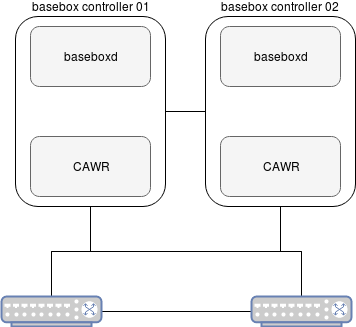
\includegraphics[width=.5\textwidth]{bisdn/basebox}
    \end{figure}
\end{frame}

\begin{frame}{Goals}
    \begin{itemize}
        \item Design and implementation of an management environment to provide an interface to develop applications 
            to manage and monitor network traffic, like
            \pause 
        \item Graphical User Interfaces (GUI), to display network topology and port statistics;

        \item monitoring \textbf{elephant flows};
    \end{itemize}
\end{frame}

\begin{frame}{Proposed Architecture}
    \begin{figure}
        \includegraphics[width=.7\textwidth]{proposed_work/proposed_system}
    \end{figure}
\end{frame}

\begin{frame}{Testing Environment}
    \begin{itemize}
        \item Due to the differences between the OF-DPA compliant hardware switches and the standard OpenFlow implementation used in the virtualised 
            network Mininet, testing the elephant flow detection mechanism proved impossible with Basebox, which led us to choosing a different controller
            \pause 
        \item The controller chosen was Floodlight, due to simplicity of installation and REST interface
        \item For development of the Graphical User Interface, the standard Basebox topology was used
    \end{itemize}
\end{frame}

\begin{frame}{Testing Environment}
    \begin{figure}
        \includegraphics[width=.7\textwidth]{meter_eleph/testing_setup}
    \end{figure}
\end{frame}

\section{Management API}

\begin{frame}{Design}
    \begin{itemize}
        \item By modifying the controllers to expose already available information like port statistics
            and link status, we created a simple GUI for simple visualization of this information

        \item Based on a Remote Process Call framework, gRPC, we leverage this protocol's serialization model
            and RPC definition to create the endpoints between the GUI client and the controllers

        \item We model the data according to standardized Yang data models, as defined by OpenConfig and IETF

        \item The GUI client is a web page based on the Django Framework
    \end{itemize}
\end{frame}

\begin{frame}{Proof-of-concept}
    \begin{figure}[!tbph]
      \centering
      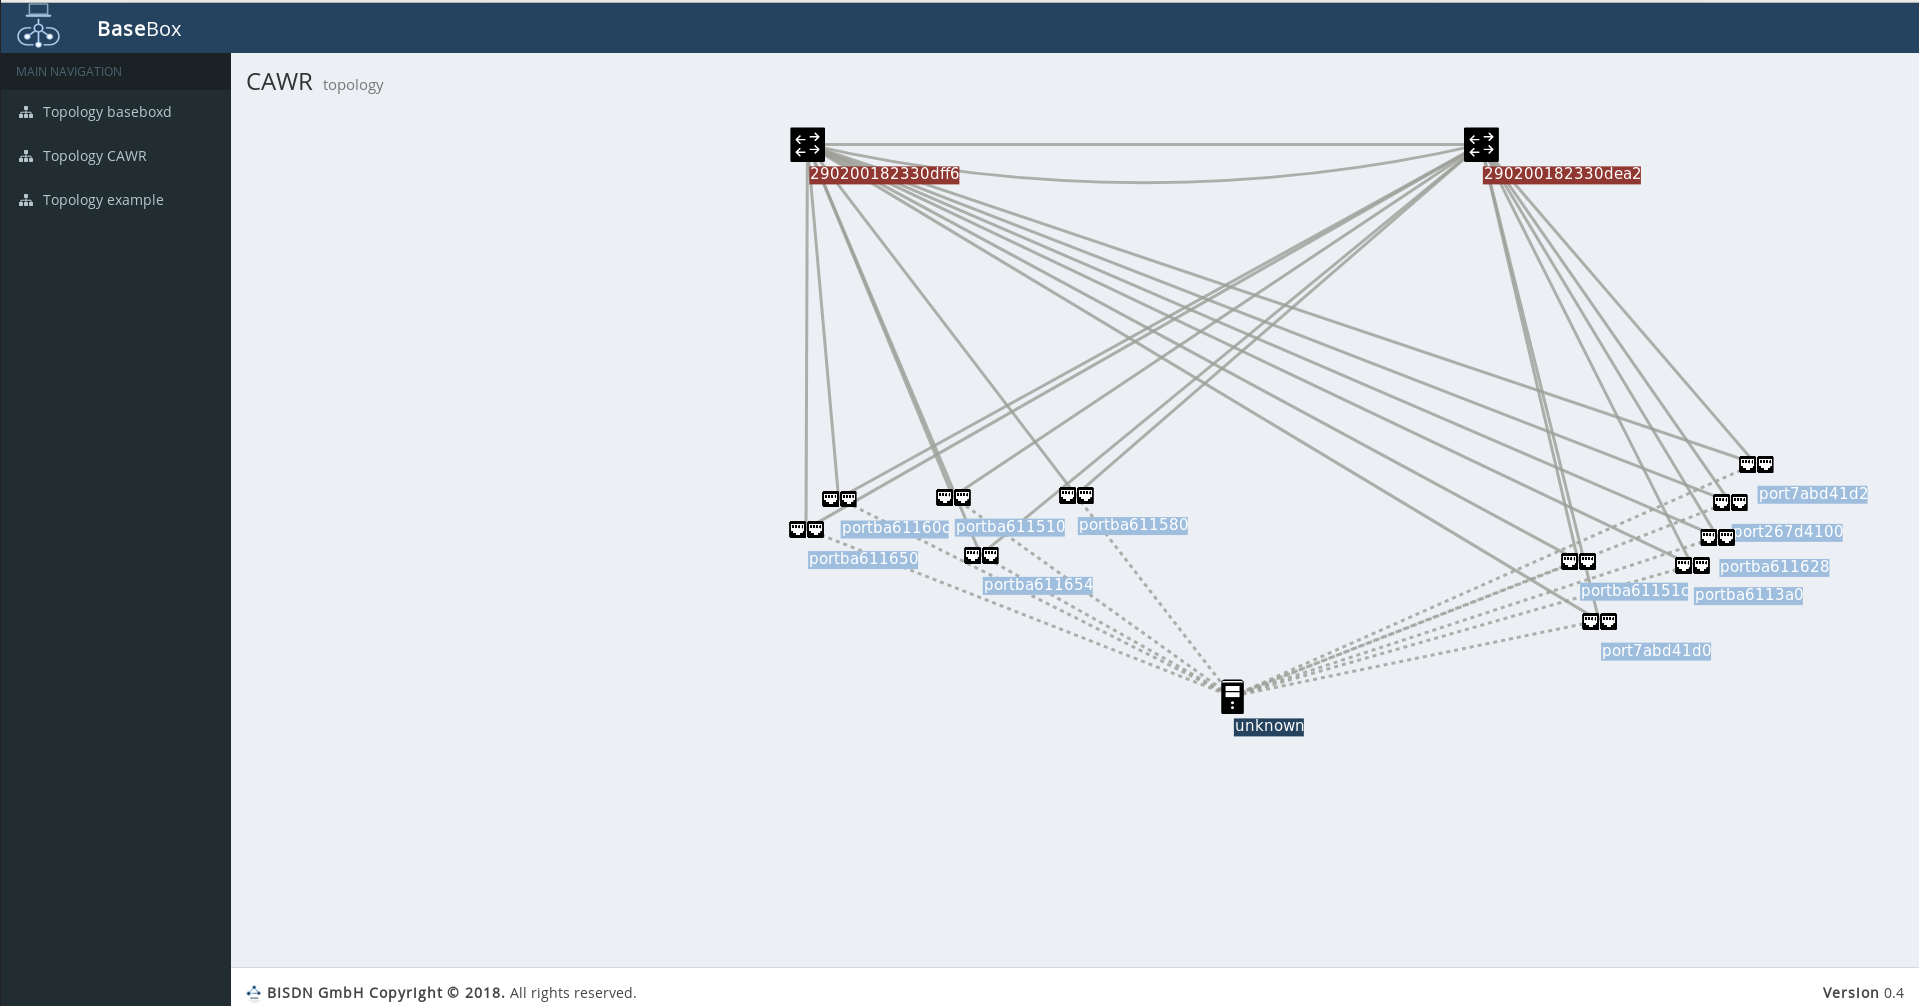
\includegraphics[width=0.8\textwidth]{bisdn/cawr_gui}
      \caption {CAWR topology, with the underlying switch topology}
    \end{figure}
\end{frame}

\begin{frame}{Proof-of-concept}
    \begin{figure}[!tbph]
      \centering
      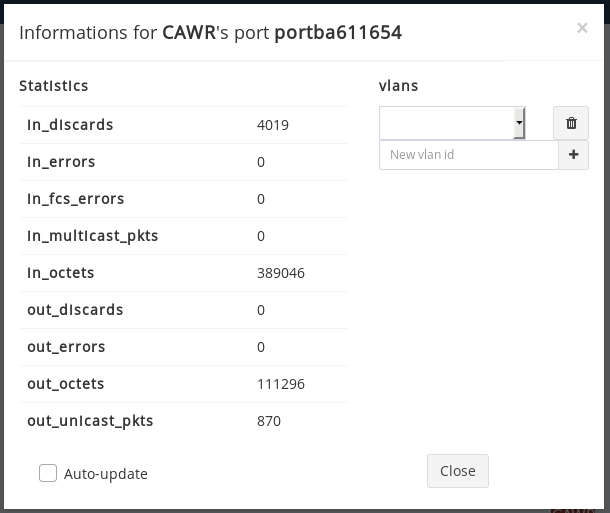
\includegraphics[width=0.7\textwidth]{bisdn/basebox_gui}
      \caption {baseboxd's statistics, with the statistics of a single port}
    \end{figure}
\end{frame}

\section{Elephant Flow Monitoring}

\begin{frame}{Proposed Algorithm}
    \begin{algorithm}[H]
        \caption{Elephant Detection Algorithm - High Level} \label{alg:high_level}
        \begin{algorithmic}[1]
            \Procedure {Elephant Flow Detection}{}
                \State Initialization
                \Loop
                    \State Query controller
                    \State Calculate the prediction error
                    \State Predict the next values
                    \State Detect the elephant flows
                    \If {Detection}
                        \State Raise Alarm
                    \EndIf
                    \State wait 2 seconds
                \EndLoop
            \EndProcedure 
           \end{algorithmic}
    \end{algorithm}
\end{frame}

\begin{frame}{Error calculation}
    \begin{figure}
        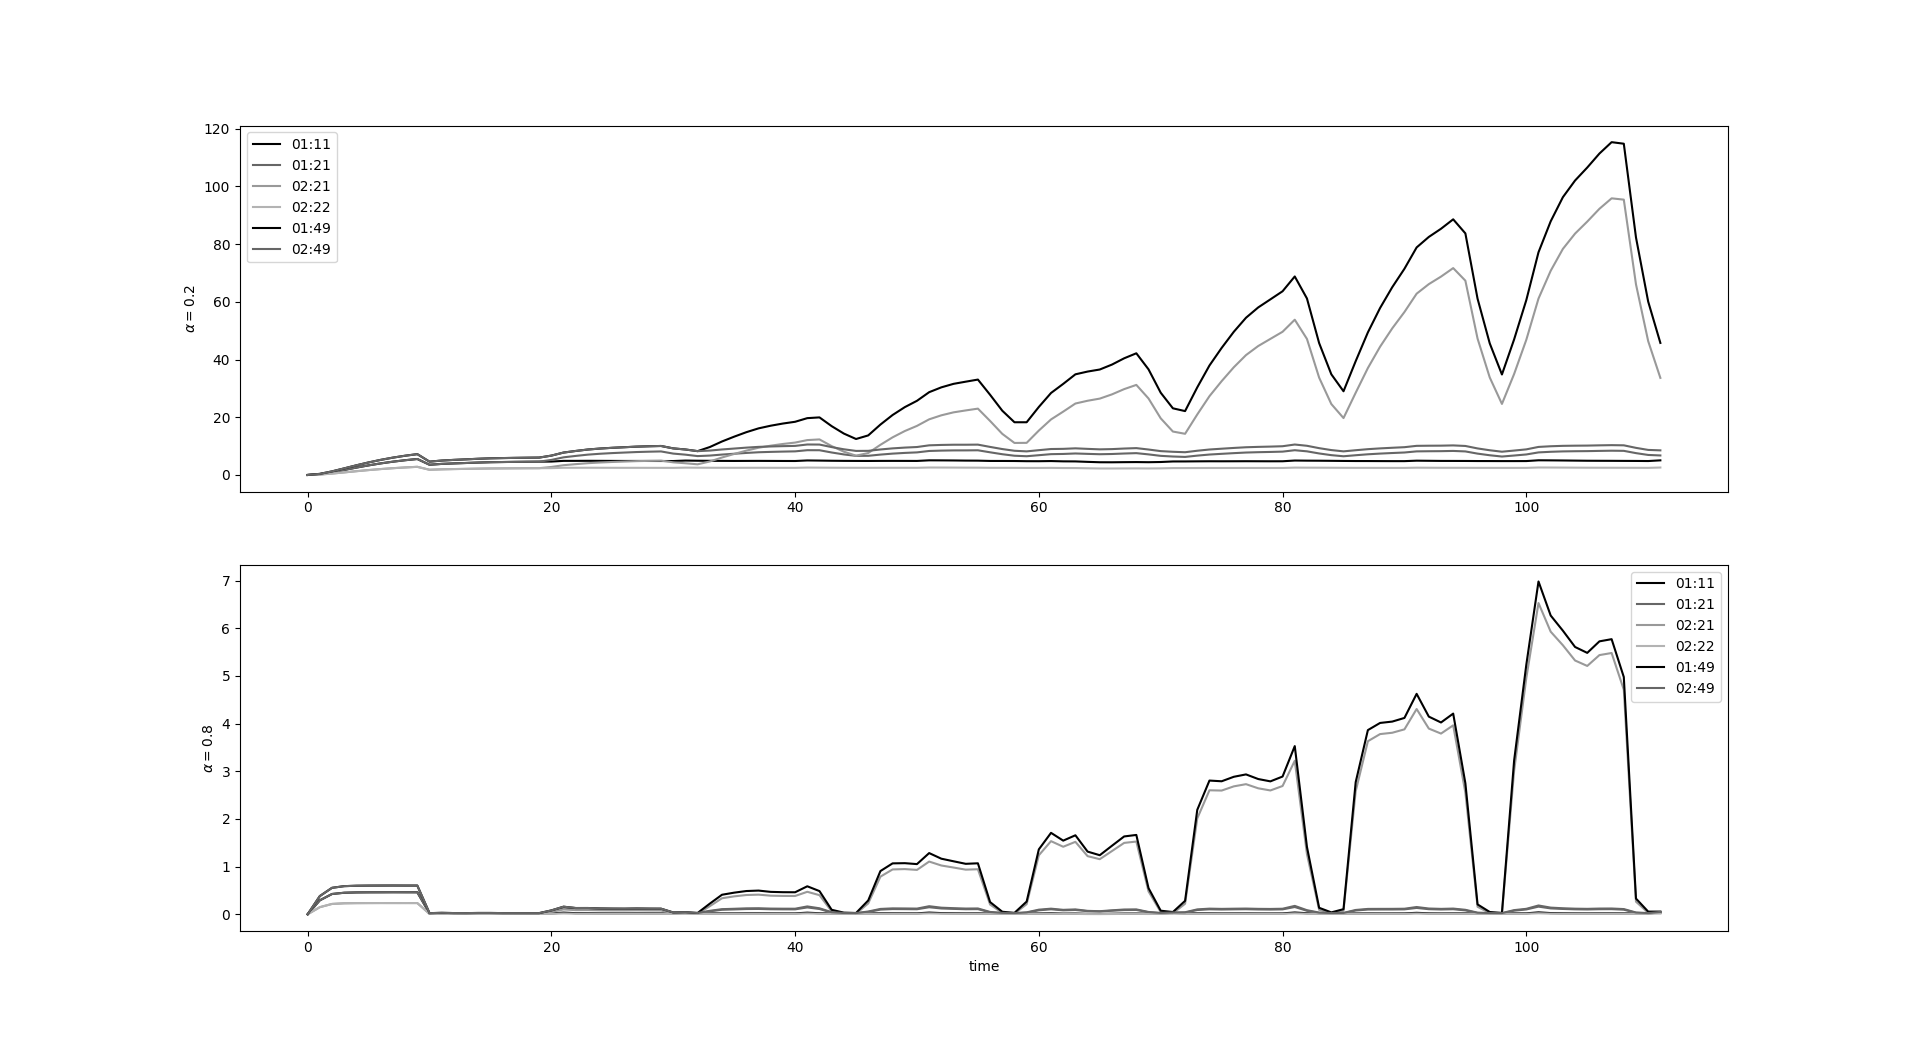
\includegraphics[width=1\textwidth]{meter_eleph/error_plot_sse}
        \caption{The prediction error obtained during the run time of the algorithm}
    \end{figure}
\end{frame}

\begin{frame}{Detection}
    \begin{figure}
        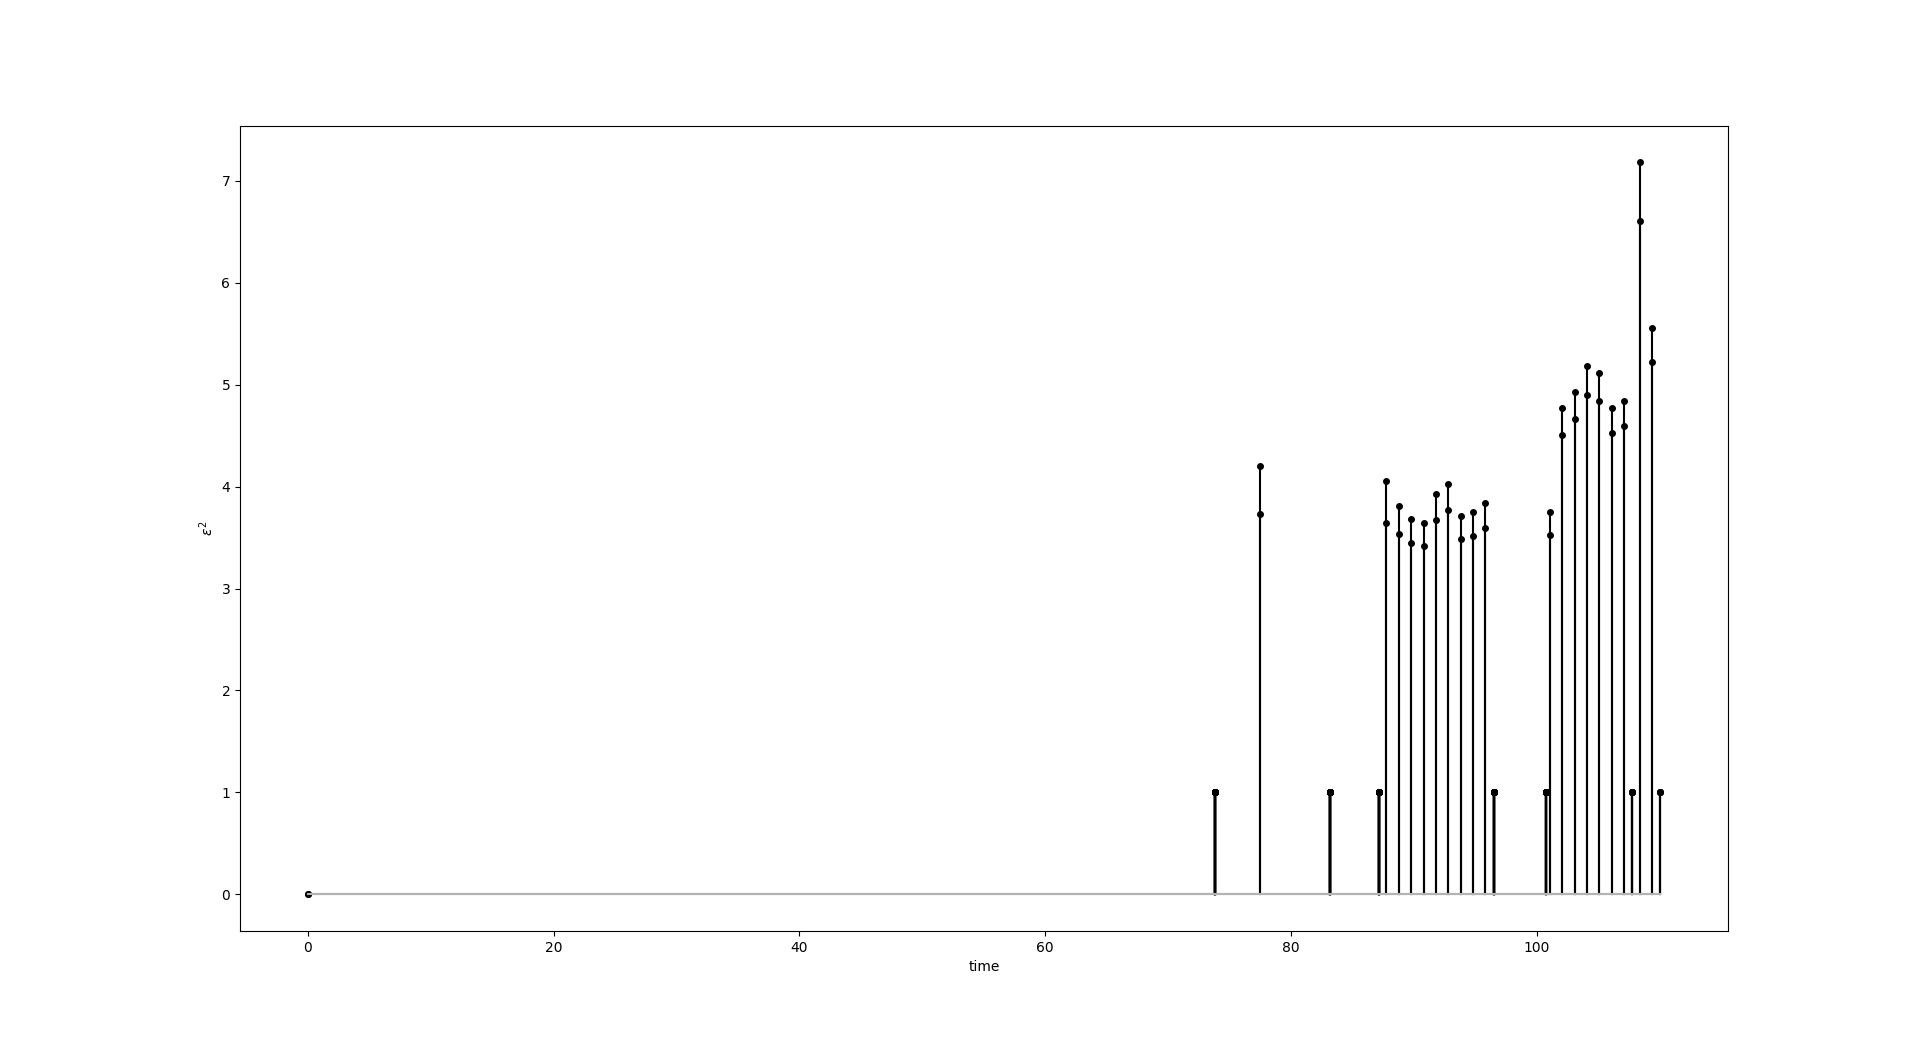
\includegraphics[width=.8\textwidth]{meter_eleph/detect_dumb}
        \caption{First detection results}
    \end{figure}
\end{frame}

\begin{frame}{Detection}
    \begin{itemize}

        \item Previous detection results are not ideal, purely comparing the output
            of a value to a pre selected threshold, and raising several alarms
            even no change has been detected


        \item The CUSUM algorithm is commonly used for change detection mechanisms employed
            in economics, health care, industrial engineering, ...
        \item Allows for keeping track of a parameter of an output of a process, and 
            compare it to pre selected thresholds, guaranteeing that the process is "in control"
    \end{itemize}

    \begin{figure}
        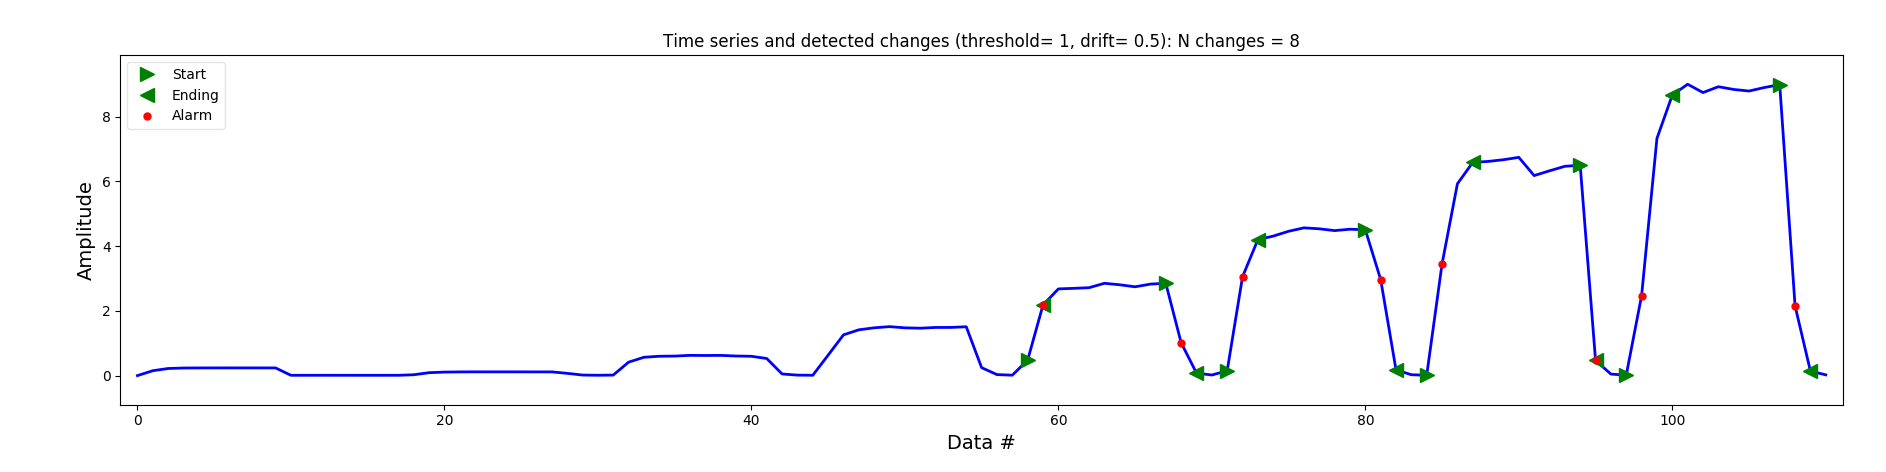
\includegraphics[width=1\textwidth]{meter_eleph/offline_cusum_output}
        \caption{Offline CUSUM output}
    \end{figure}
\end{frame}

\begin{frame}{Detection}
    \begin{itemize}
        \item Adaptation of the CUSUM algorithm to an online context is based on a sliding window
            method 
    \end{itemize}

    \begin{figure}
        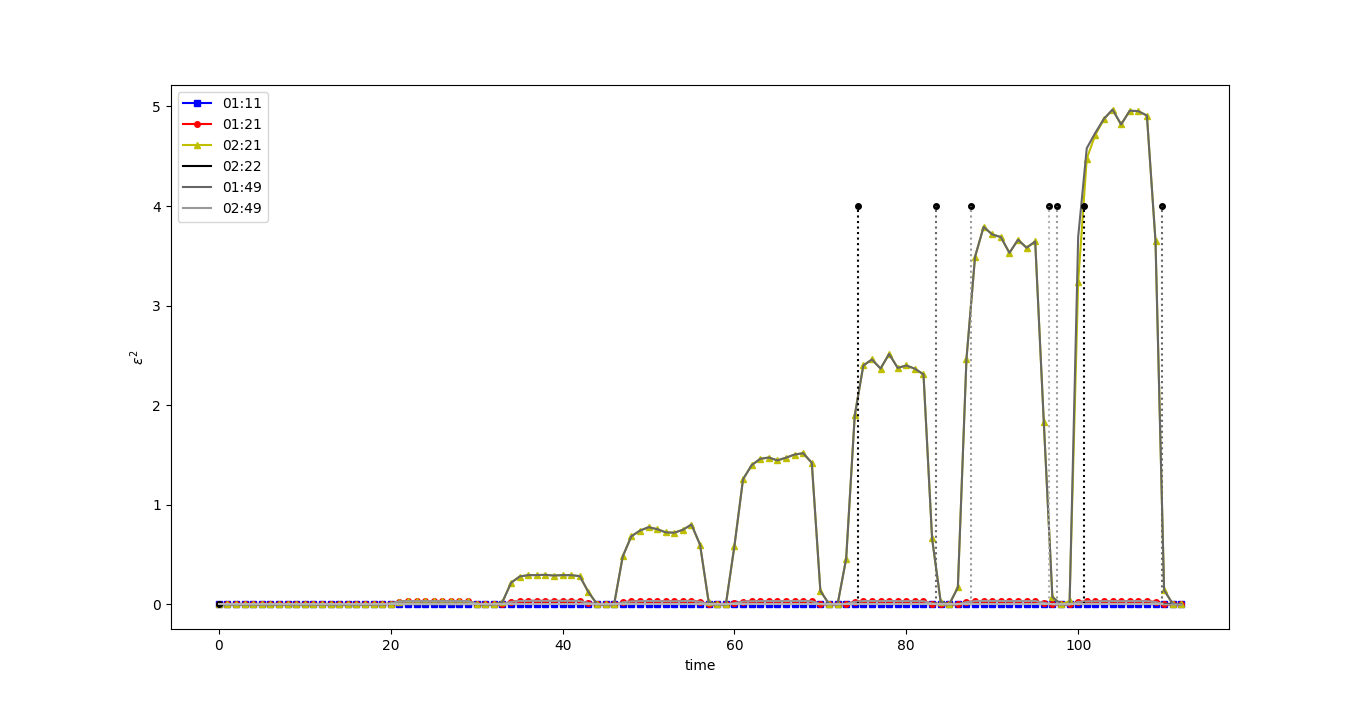
\includegraphics[width=.6\textwidth]{meter_eleph/detection_results_plotted}
        \caption{Online CUSUM output}
    \end{figure}
\end{frame}

\begin{frame}{Detection}
    \begin{figure}
        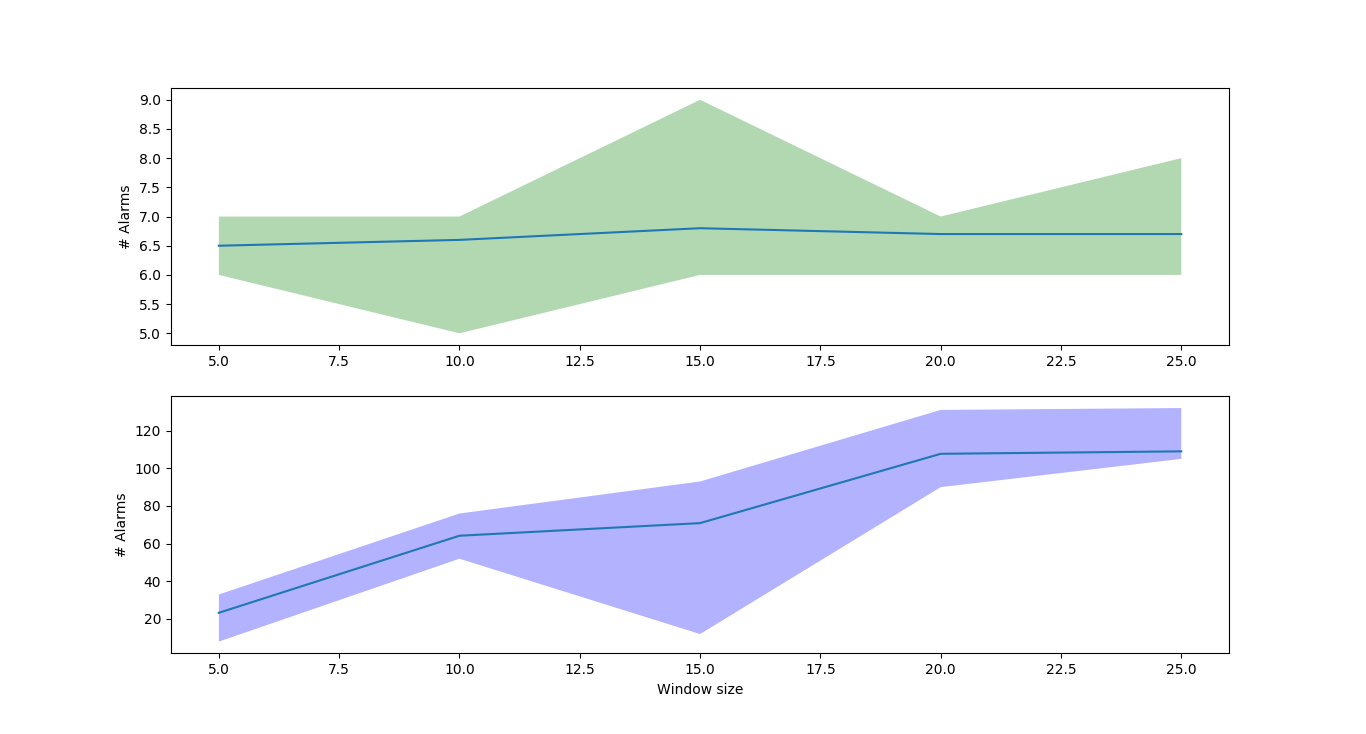
\includegraphics[width=.7\textwidth]{meter_eleph/evaluation_error}
        \caption{Comparison of the number of alarms raised by the enhanced (top) and non enhanced (bottom) versions}
    \end{figure}
\end{frame}

\begin{frame}{Detection}
    \begin{figure}
        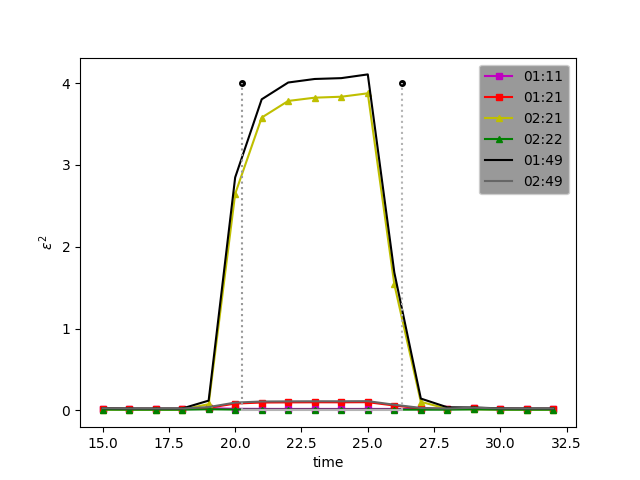
\includegraphics[width=.9\textwidth]{meter_eleph/single_elephant_flow}
        \caption{Single Elephant Flow}
    \end{figure}
\end{frame}

\begin{frame}{Evaluation of detection algorithm}
    \begin{figure}
        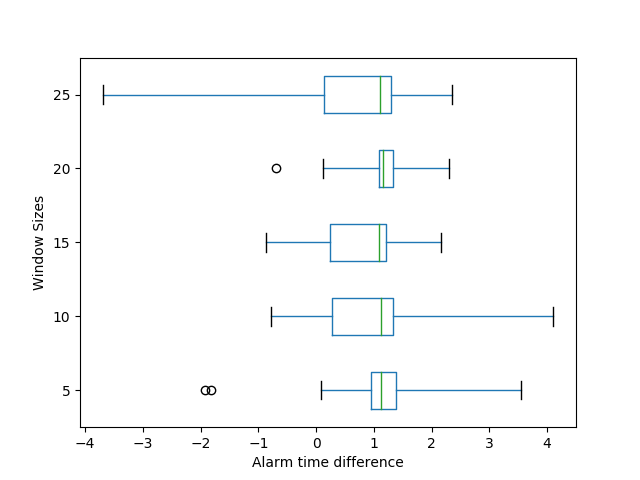
\includegraphics[width=.7\textwidth]{meter_eleph/time_error}
        \caption{Detection time difference for different window sizes}
    \end{figure}
\end{frame}

\begin{frame}{Evaluation of detection algorithm}
    \begin{table}[]
        \centering
        \caption{False alarms statistics}
        \label{tab:false_alarms}
        \begin{tabular}{|c|c|c|c|c|c|}
            \hline
            Window Size   & 5        & 10       & 15  & 20  & 25  \\ \hline
            count         & 30       & 30       & 30  & 30  & 30  \\ \hline
            $\bar{x}$            & 2.833333 & 2.166667 & 2.0 & 2.0 & 2.0 \\ \hline
            $\sigma^2$& 0.791478 & 0.379049 & 0.0 & 0.0 & 0.0 \\ \hline
        \end{tabular}
    \end{table}
\end{frame}

\section{Conclusion}

\begin{frame}{Summary of Achievements}
    \item We have proposed and implemented a system that
    \begin{itemize}
        \item integrates a Software-Defined Controller environment, and exposes internal
            management information

        \item allows the development of management applications, that we have proven 
            by developing a Proof-of-Concept containing on a Graphical User Interface

        \item extends the controllers capability for monitoring network traffic, 
            by analysing traffic statistics for elephant flow detection
    \end{itemize}
\end{frame}

\begin{frame}{Future Work}
    \begin{itemize}
        \item Extend the GUI for displaying VLANs and layer 3 information like routes and neighbours;
        \item Extend the traffic change monitoring for closer insights on possible offending flows;
        \item Research the capacity that the controllers have for implementation of OpenFlow meters,
            allowing us to shape individual traffic flows.
    \end{itemize}
\end{frame}

\begin{frame}{Achievements}
    \begin{figure}
        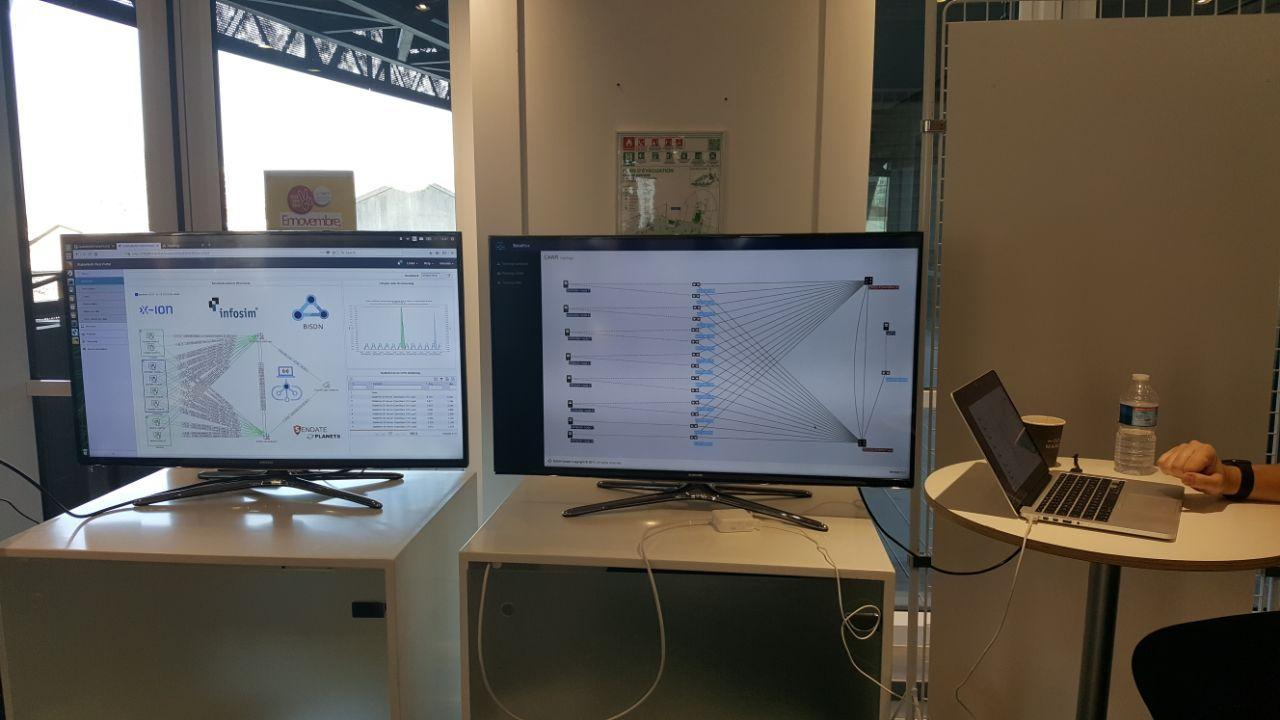
\includegraphics[width=.9\textwidth]{presentation/basebox_paris}
        \caption{Image of the developed GUI, present in the SENDATE Mid Term Event in Paris}
    \end{figure}
\end{frame}

\printbibliography
\end{document} 
%\begin{frame}{}
%\end{frame}
